\section{量子力学中的本征值问题}
与量子化学有关的数学和物理,几乎没有例外,都是面向求解一类特殊问题,即用组成体系的粒子的基本性质(电荷,质量)计算分子体系的性质。
只用电子电荷,普朗克常数等计算分子中电子的能量就是一个很好的例子。
读者或已知道这个问题的答案的本性\footnote{个人感觉翻译成本质更好}了。
分子中的电子的能量可取一些分立值,但当能量的值高达某一点后再高的能量值则在连续区中。
这些能值定性地示于图1-1中。
正如实验指出的那样,量子力学为某些物理量提供的结果是它们只能取某些值而非全部值。
一物理量的许可值称为本征值,他来源于德语特征值。
一特殊物理量的本征值可取值于连续区或取自有限或无线的一组分立本征值中。
例如,一个原子的能量可以是无限多个分离本征值中的一个,也可以是更高区中的称为连续谱的本征值中的一个。
化学设计的物理量多半是分立本征值而非连续本征值\footnote{大概是由于基本在处理电子态处于基态时的分子。}。
\begin{figure}[htbp]
    \center
    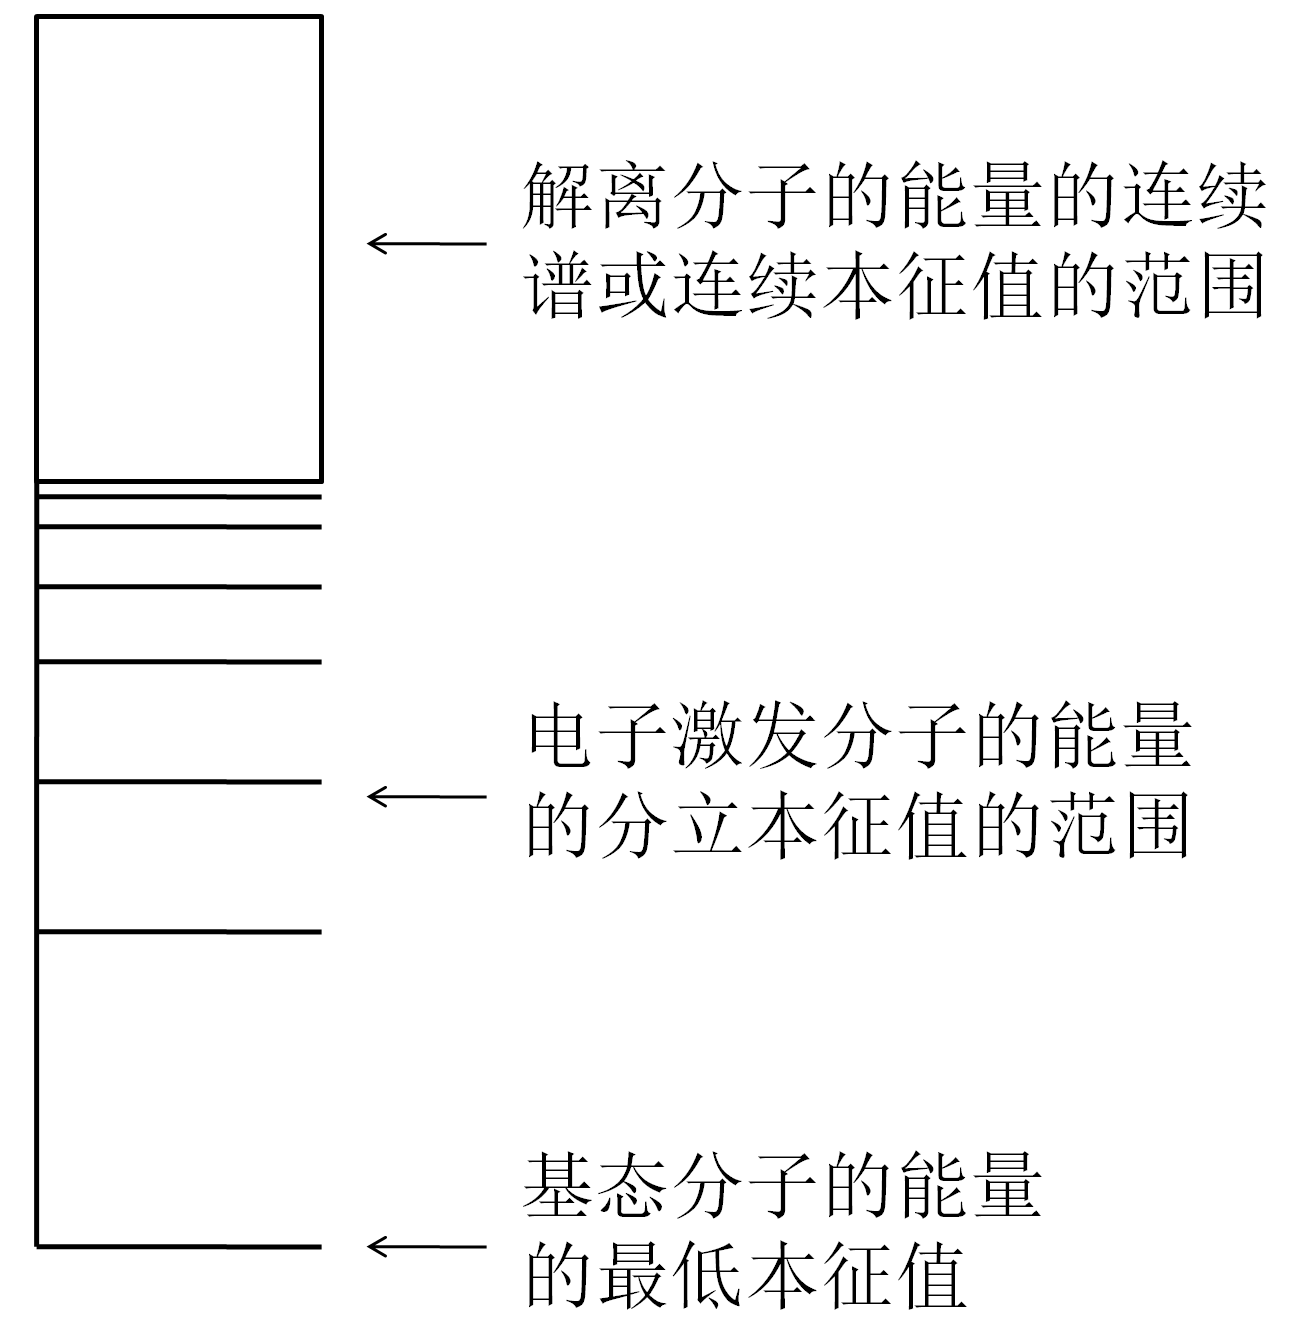
\includegraphics[scale=0.15]{./fig/1-1.png}
    \caption{分子的能量的本征值}
\end{figure}
求一物理量的本征值的数学问题称为本征值问题;用通常称为本征值方程的那种形式的方程计算。
一物理量Q的本征值方程具有易为人误解的简单外观:
\[\hat{Q}f=qf \tag{1-1}\]
方程中f是一函数,称为物理量Q具有本征值q的本征函数。符号$\hat{Q}$称为算符,$\hat{Q}f$这个陈述式告诉我们如何将函数f按$\hat{Q}$的定义中的含义所指出的那样换成一个新函数。
本征值方程(方程1-1)表示将算符$\hat{Q}$所示的那些规则用于f得到的函数是原来函数f的q倍。
很值得提出的一种情况是几根本征函数具有相同的本征值;即$\hat{Q}f_1=qf_1$,$\hat{Q}f_2=qf_2$等等。
在此情况下可称q是简并\footnote{原文中“简bing”的bing为“左伴随”单人旁的“并”,在LaTeX中打不出来,故用“并”代替}的,具有相同本征值的本征函数的数目叫做简并度。

算符可以只是数或函数;例如,可定义算符X为“对被运算函数乘以x”;因此$Xx^2=x^3$。
另一方面,算符可以比数或函数更复杂些。
例如,同学们已经使用过的下述算符(虽未用算符这个名称),它表示或定义为“求某变量的改变”。
例如$\Delta$作用于热力学函数H(焓)得到新函数$\Delta H$(焓的改变),$\Delta H=H_2-H_1$。
人们熟悉的另一算符是$\dv{x}$,他用于表示“对x求导数”。

如何写出对应于欲测物理量的算符是量子力学的任务。
目前我们的任务是学习如何求解这类算符的本征值方程,特别是学习用于讨论方程的解的性质的词汇和概念。
而量子力学本身是从两个不同的观点发展起来的,这两种观点代表本征值问题的两个类似的数学处理。

第一个观点是薛定谔的波动力学。
在波动力学里,算符是微分表达形式,像前边提到的算符$\dv{x}$那样,因而本征值方程区微分方程形式,可应用微积分学求解。
第二个表述是海森堡的矩阵力学,在矩阵力学中算符表示成叫做矩阵的代数形式;代替本征值方程中是函数,矩阵算符作用于向量$\zeta$将$\zeta$变换为与$\zeta$平行的向量,后者的长度是$\zeta$的q倍。
\[\hat{Q}\zeta=q\zeta \tag{1-2}\]
方程1-2是本征值问题的矩阵力学陈述形式。
在第三章中将对矩阵和向量给予定义并作详细讨论。
如方程1-1那样,q是物理量Q的本征值,$\zeta$是本征向量,$\hat{Q}$是用矩阵表述的算符。
这种形式的本征值问题的求解是用代数学。

量子力学的这些表面上不同的数学和物理处理方法,实际上有着深刻的相互联系;狄拉克的工作证明了两种观点的内在等价性,也证明了对应的数学技巧的内在等价性。

\section{经典力学的本征值问题}
我们已经简要地讨论了量子力学中本征值方程的作用。
但经典力学中的一些问题也可以用简单而有意义的方式表示为本征值问题。
其中力学体系(如分子)的振动和转动就是这类问题。
这些物理问题对研究分子运动和光谱学的化学家很重要。
在振动中,振动的简正方式和频率可表现为本征向量和本征值;在转动中,从本征值问题中可以得出主轴和惯性矩。
但应注意,在分子水平上正确地描述这些体系,总是需要量子力学,而非经典力学。

\section{本书涉及的范围}
根据我们希望能提出的,求解的和理解的问题的种类决定了的要求,在本课程中先学习与本征函数密切相关的一类函数,然后学习向量代数和矩阵代数,最后将本征值问题的两种观点综合起来。
并用经典力学的研究收尾,即了解如何将力学体系(如分子)的振动表示为本征值问题。同时试图将牛顿力学以它与量子力学的关系很清晰的形式表示出来\footnote{这里感觉作者翻译得有问题,我猜大概是想表达“同时试图将牛顿力学与量子力学之间的关系以很清晰的方式表达出来”}。

我将沿此途径学习本征值问题的一些方法,并采用一些化学中感兴趣的应用。
我们的着重点始终是概念第一,方法第二,而将数学定理的详细证明放在最次要的地位。
在每章后给出一组习题。
许多习题的答案和提示放在全书的后面。

\begin{problemset}
    \item 求算符$\dv{x}$的本征函数。
\end{problemset}